\documentclass[tikz]{standalone}

\begin{document}
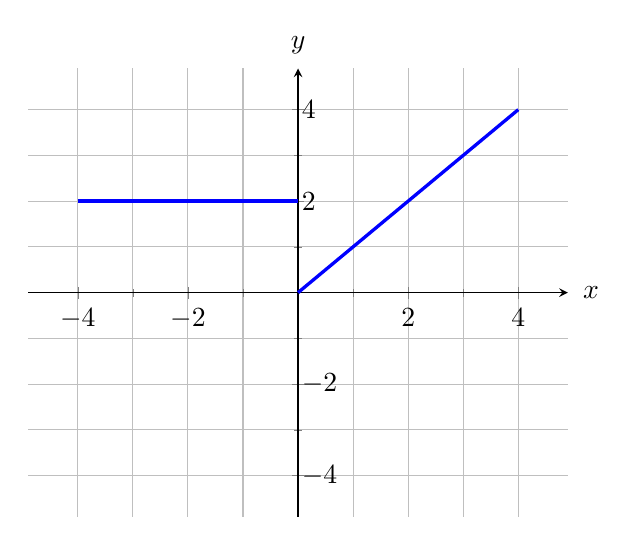
\begin{tikzpicture}
    \begin{axis}[%
        xlabel=$x$, ylabel=$y$, legend pos=south east,
        grid=both, xmin=-4.9, xmax=4.9, ymin=-4.9, ymax=4.9,
        axis lines = middle,
        minor x tick num=1, minor y tick num=1,
        xlabel style = {at={(axis description cs:1.01,0.5)},anchor=west},
        ylabel style = {at={(axis description cs:0.5,1.01)},anchor=south},
        % xticklabels = {}, yticklabels = {},
        yticklabel style = {right},
    ]
    % \draw[thick, dashed,] (-4,2.5) -- (-4,0) node[below]{$-4$}
    %     (4.5,{3/2}) -- (4.5,0) node[below]{$4.5$}
    %     (7,{2/3}) -- (7,0) node[below]{$7$}
    %     (-1,2.5) -- (0,2.5) node[right]{$2.5$}
    %     (0,-2) node[left]{$-2$} -- (2,-2)
    %     (-1,2.5) -- (-1,0) node[below]{$-1$};
    \addplot [blue, mark=none, domain=-4:0, very thick] plot {2};
    \addplot [blue, mark=none, domain=0:4, very thick] plot {x};
    \end{axis}
\end{tikzpicture}
\end{document}
